\documentclass{article}
\usepackage{booktabs}
\usepackage[UTF8]{ctex}
\usepackage{enumitem}
\usepackage{graphicx}
\usepackage{float}
\usepackage{subfigure}
% \usepackage{amsmath}
\usepackage{amsmath,amsfonts}
\usepackage{hyperref}

\begin{document}
\sloppy % 解决中英文混排的断行问题

\title{环境感知犯罪事件预测}
\author{郑泓东 21311570,黄裔杰21311571}
\date{\today}

\maketitle

\renewcommand{\abstractname}{摘要}  % 更改摘要名称

\begin{abstract}
    本实验旨在通过机器学习方法对洛杉矶的犯罪情况进行预测。我们使用了洛杉矶市历史犯罪数据集(2020-2023),并采用了多种算法(例如逻辑回归、多层感知机和决策树等)来构建预测模型。我们将数据集划分为训练集和测试集,通过评估模型在测试集上的性能来验证预测模型的准确性。本实验的初衷是为亲爱的洛杉矶居民提供一个赛博算命的方法,根据此时此刻的环境信息(月份、日期、小时、分钟、地区、年龄、性别、种族、经纬度)来预测未来可能遭遇的犯罪类型、武器类型、犯罪地点以及案件状态,以便居民采取相应的措施来保护自身安全。
\end{abstract}

\section{引言}
犯罪预测是应用机器学习和数据分析的一个重要领域。通过分析历史犯罪数据,我们可以识别出与犯罪相关的模式和趋势,并利用这些信息来预测未来可能发生的犯罪事件。这种预测能力可以帮助居民避免潜在的危险,保护自身安全。

\section{数据预处理}
我们使用的数据集\href{https://www.kaggle.com/datasets/asaniczka/crimes-in-los-angeles-2020-2023/data}{ Los Angeles Crime Data 2020-2023 }来自 Kaggle \footnote{\href{https://www.kaggle.com/}{Kaggle}:一个数据科学竞赛和社区平台。该平台提供了丰富的数据集供研究和分析使用。}。该数据集包含了多个属性,包括 division\textunderscore{}number(犯罪事件的分区编号)、date\textunderscore{}reported(报告犯罪的日期)、date\textunderscore{}occurred(犯罪发生的日期)、area(犯罪事件发生地的区号)等27个属性(图\ref{fig:Details})。在预处理阶段,我们对数据进行了清洗和转换。这包括处理缺失值、转换日期和时间格式。

\begin{figure}[H]
    \centering
    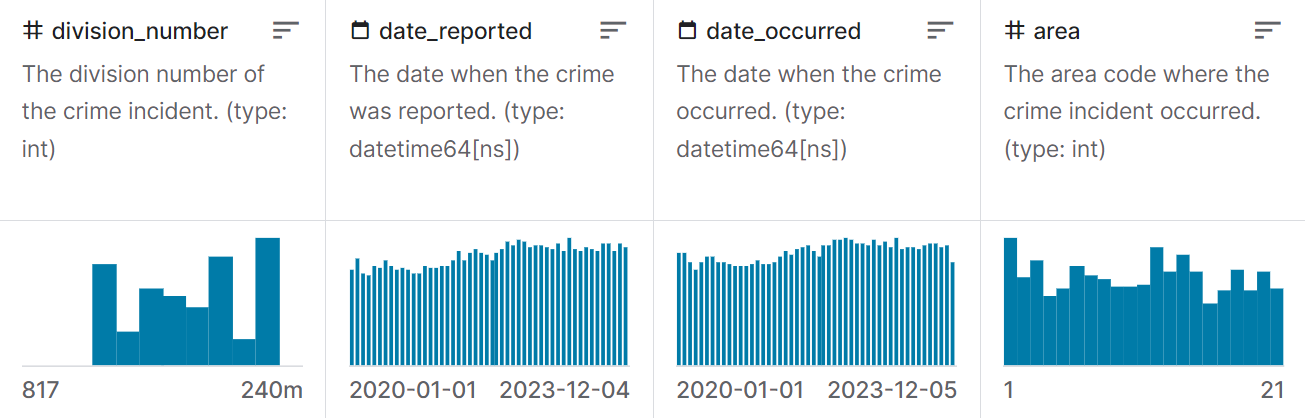
\includegraphics[width=1\textwidth]{../pic/Screenshot 2024-01-12 111029.png}
    \caption{Details of the dataset}
    \label{fig:Details}
\end{figure}

\section{特征选择}
在构建预测模型之前,我们首先进行了特征选择。本实验是用已知的环境信息,预测未知的犯罪事件,因此,不是所有的特征都对预测犯罪事件是有用的。一种是犯罪事件发生之后记录的信息,如 division\textunderscore{}number(犯罪事件的分区编号)、date\textunderscore{}reported(报告犯罪的日期)、reporting\textunderscore{}district(犯罪事件的报告地区)等;另一种是映射关系如 area(犯罪事件发生地的区号)对应的 area\textunderscore{}name(犯罪事件发生的地区名称)。我们认为这些信息对于预测犯罪事件是没有意义的,因此我们将这些特征从数据集中删除。

我们选择了一组与犯罪预测相关的特征,例如 date\textunderscore{}occurred(犯罪发生的日期)、area(犯罪事件发生地的区号)、crime\textunderscore{}code(犯罪类型对应的代码)、victim\textunderscore{}age(受害人的年龄)等。这些特征可以用来描述犯罪事件的犯罪类型、时间、地点等,具有较高的信息量。

\subsection{犯罪事件的时间和空间分布}
我们将数据按照 area 分组,以经纬度均值作为该区域的中心点,绘制了犯罪事件的地理分布图(图\ref{fig:map})。犯罪数量排前三的区域分别是 77th Street、Central 和 Southeast。

\begin{figure}[H]
    \centering
    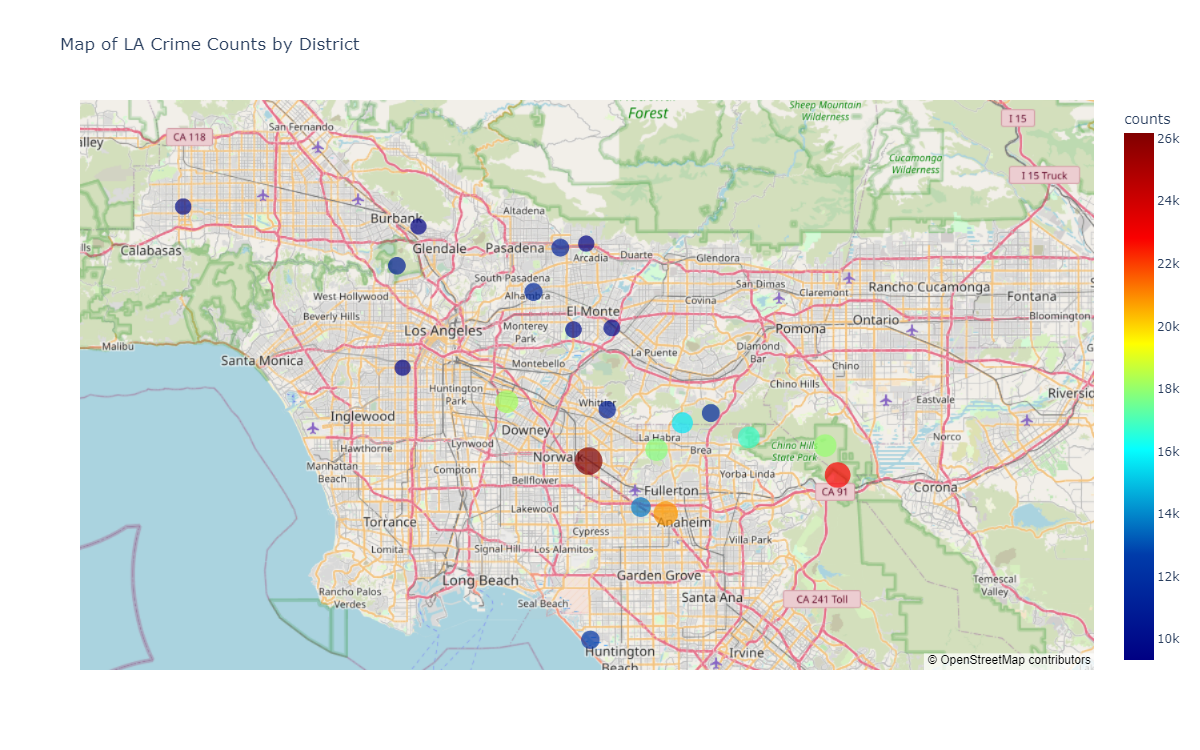
\includegraphics[width=1\textwidth]{../pic/map.png}
    \caption{Map of LA Crime Counts by District}
    \label{fig:map}
\end{figure}

我们还绘制了犯罪事件与日期、月份(图\ref{fig:date})以及小时(图\ref{fig:hour})的关系。从图中可以看出,犯罪事件的数量在一年中的不同月份和一天中的不同时间段有所不同。例如,犯罪事件在夏季和秋季较多,而在冬季较少。此外,犯罪事件在下午和晚上较多,而在凌晨较少。有趣的是,犯罪事件在每个月的前几天较多,其它时间较为平均。

\begin{figure}[H]
    \centering
    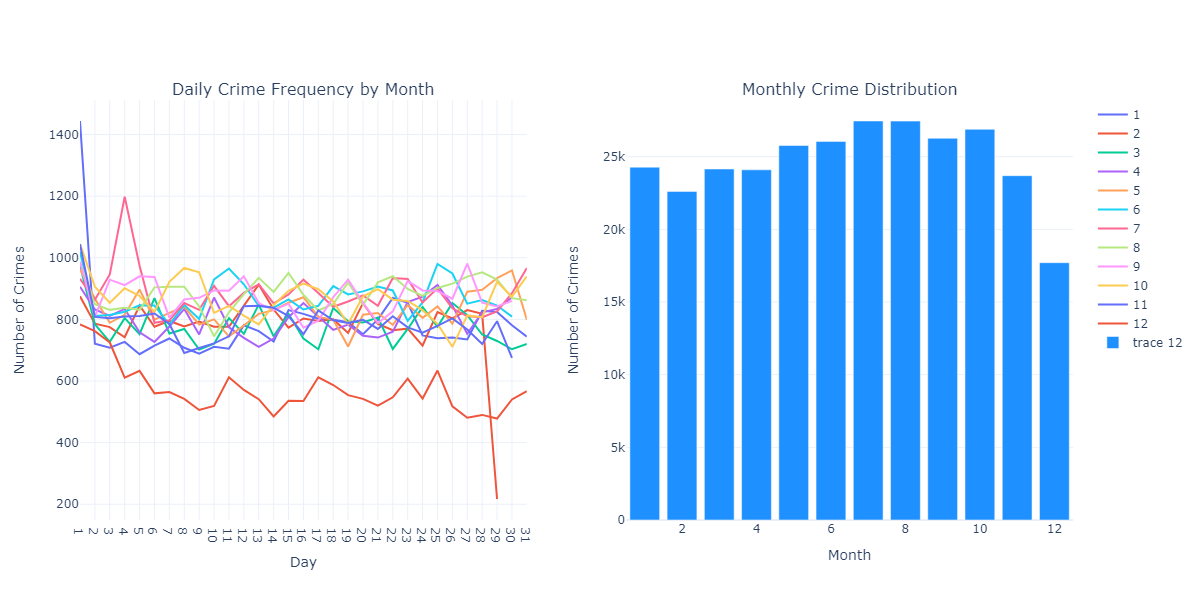
\includegraphics[width=1\textwidth]{../pic/date.png}
    \caption{Daily Crime Frequency by Month and Monthly Crime Distribution}
    \label{fig:date}
\end{figure}

\begin{figure}[H]
    \centering
    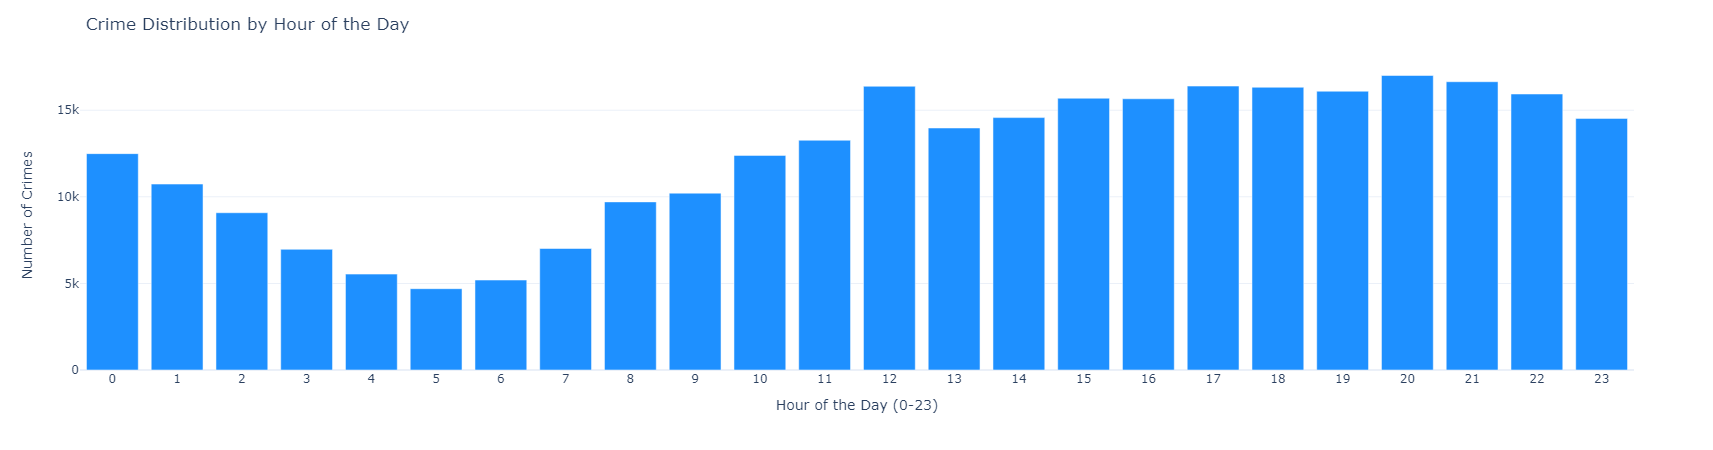
\includegraphics[width=1\textwidth]{../pic/hour.png}
    \caption{Crime Distribution by Hour of the Day}
    \label{fig:hour}
\end{figure}

\subsection{受害人信息及处理}
我们统计了受害人的年龄,并使用随机采样,针对每个无效年龄(0或负值),随机选择一个有效年龄值来替代(图\ref{fig:age}为处理前后),这种方法可以更好地保持数据分布。从图中可以看出,受害人的年龄集中分布在20-39岁。

\begin{figure}[htbp]
    \centering

    \subfigure[Distribution of Victim Age before processing]{
        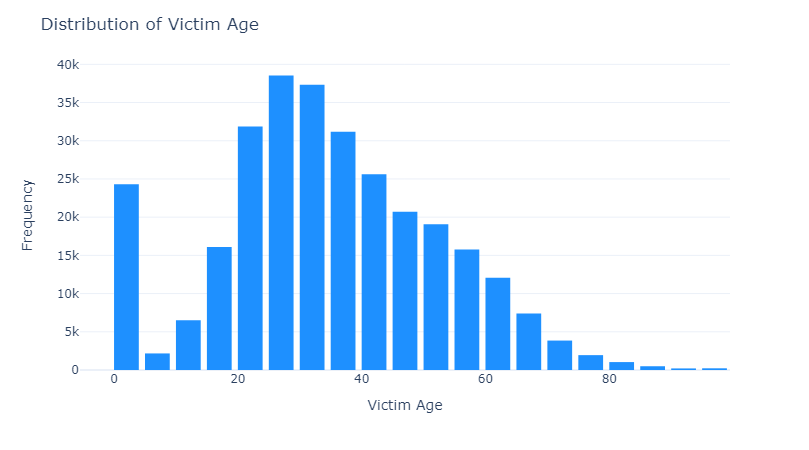
\includegraphics[width=0.4\textwidth]{../pic/age_before.png}
        \label{fig:age_before}
    }
    \hspace{0.5cm}
    \subfigure[Distribution of Victim Age after processing]{
        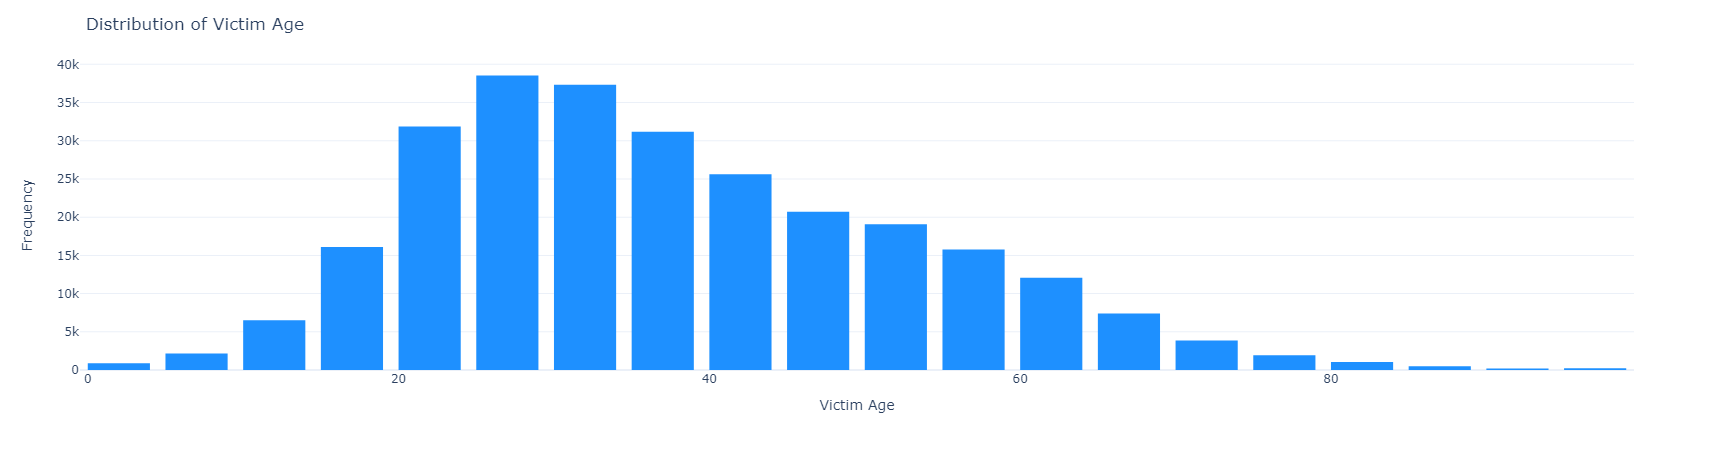
\includegraphics[width=0.4\textwidth]{../pic/age_after.png}
        \label{fig:age_after}
    }

    \caption{Distribution of Victim Age}
    \label{fig:age}
\end{figure}

受害人的性别分布中(图\ref{fig:sex_and_descent}左侧),男性和女性占大多数,少部分属于未知性别。而种族分布中(图\ref{fig:sex_and_descent}右侧),H(西语裔\footnote{西语裔:通常指拉丁美洲或西班牙裔。})遥遥领先,其次是B(非裔美国人),再次是W(白人,欧洲裔)。

\begin{figure}[H]
    \centering
    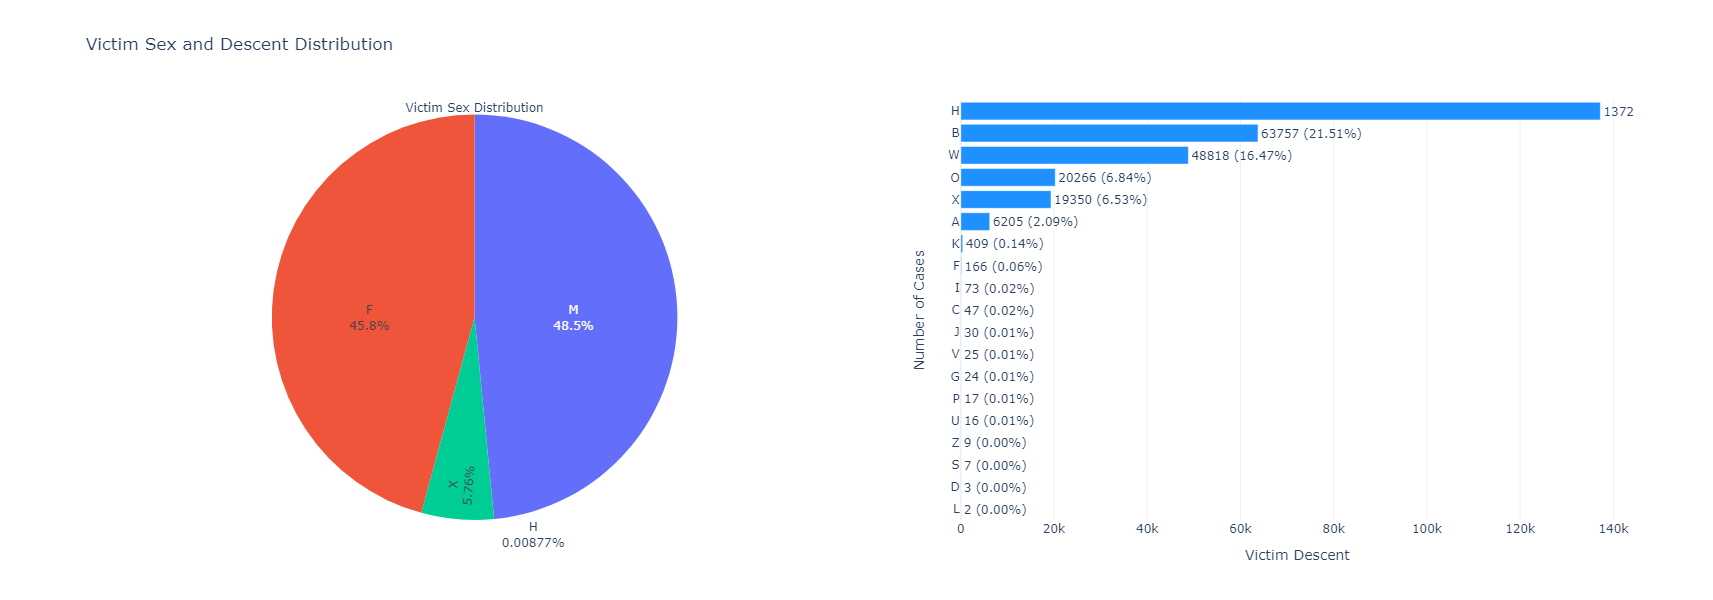
\includegraphics[width=1\textwidth]{../pic/sex_and_descent.png}
    \caption{Victim Sex and Descent Distribution}
    \label{fig:sex_and_descent}
\end{figure}

\subsection{犯罪详情 Top 10}
此外,我们还统计了犯罪事件的描述、使用的武器、犯罪发生的地点以及犯罪事件的状态,并绘制了它们的分布图(图\ref{fig:top10})。从图中可以看出,犯罪事件的描述中,最多的是“BATTERY - SIMPLE ASSAULT”(电池 - 简单攻击),其次是“ASSAULT WITH DEADLY WEAPON, AGGRAVATED ASSAULT”(使用致命武器进行攻击,严重攻击);最常用的武器是“STRONG-ARM (HANDS, FIST, FEET OR BODILY FORCE)”(强力武器);,其次是“VERBAL THREAT”(口头威胁);最常见的犯罪地点是“STREET”(街道),其次是“SINGLE FAMILY DWELLING”(单户住宅);最常见的犯罪状态是“Invest Cont”(调查中),其次是“Adult Other”(成年人案件且未被逮捕)。

\begin{figure}[H]
    \centering
    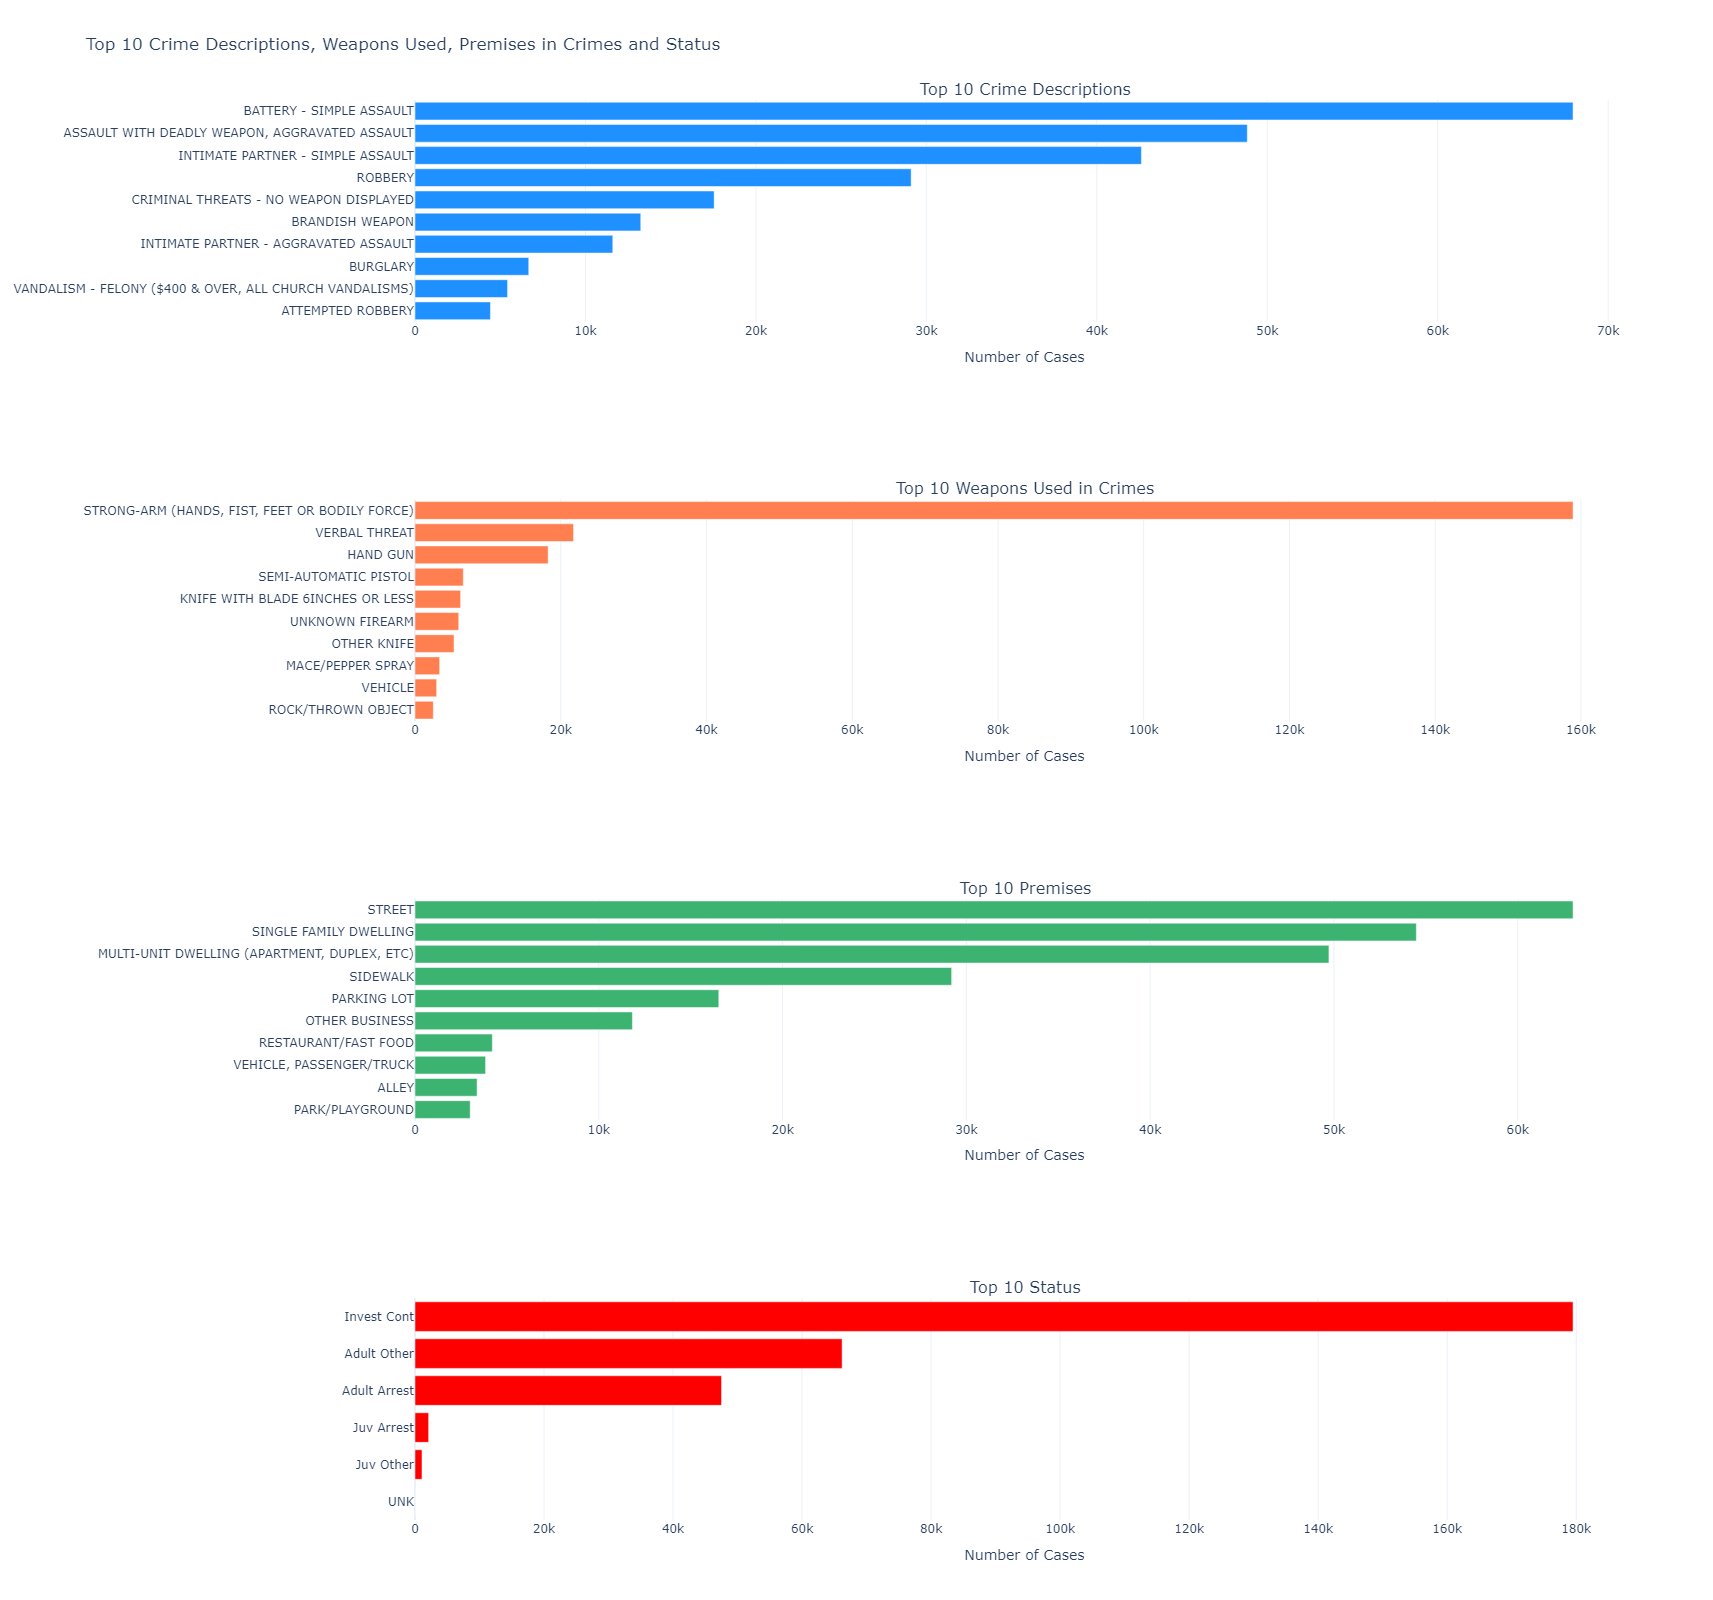
\includegraphics[width=1\textwidth]{../pic/top10.png}
    \caption{Top 10 Crime Descriptions, Weapons Used, Premises in Crimes and Status}
    \label{fig:top10}
\end{figure}

\section{模型构建与训练}
我们采用了多种算法来构建预测模型。在这个实验中,我们选择了逻辑回归作为我们的基础模型。逻辑回归是一种简单而强大的回归算法,可以根据特征的值进行预测,并生成一个逻辑方程来表示预测过程。我们还尝试了其他算法,如多层感知机、决策树和朴素贝叶斯等,以比较它们的性能(表\ref{tab:Performance})。

我们将数据集划分为训练集和测试集,采用80\%的数据作为训练集,20\%的数据作为测试集。然后,我们使用训练集来训练模型,并通过测试集评估模型的性能。衡量模式性能的指标为准确率(accuracy)。

\begin{table}[H]
    \centering
    \begin{tabular}{|c|c|c|c|c|}
        \hline
                            & crime\textunderscore{}code & premise\textunderscore{}code & weapon\textunderscore{}code & status \\
        \hline
        Logistic Regression & 0.28                       & 0.27                         & 0.54                        & 0.61   \\
        \hline
        MLP                 & 0.28                       & 0.27                         & 0.54                        & 0.61   \\
        \hline
        k-NN                & 0.22                       & 0.22                         & 0.47                        & 0.51   \\
        \hline
        Naive Bayes         & 0.03                       & 0.02                         & 0.04                        & 0.23   \\
        \hline
        Decision Tree       & 0.19                       & 0.26                         & 0.35                        & 0.48   \\
        \hline
        Classifier Chain    & 0.19                       & 0.26                         & 0.35                        & 0.48   \\
        \hline
    \end{tabular}
    \caption{Performance of different algorithms}
    \label{tab:Performance}
\end{table}

\section{实验结果与讨论}
在我们的实验中,Logistic Regression 模型和 MLP 模型表现出较好的性能。在测试集上,我们获得了约54\%的武器类型准确率(表\ref{tab:classification_report_weapon})以及60\%的案件状态准确率(表\ref{tab:classification_report_status})。对于 weapon\textunderscore{}code 来说,Logistic Regression 模型在类别61\footnote{武器类型61:STRONG-ARM (HANDS, FIST, FEET OR BODILY FORCE)}上表现较好;对于 status 来说,Logistic Regression 模型在类别3\footnote{案件状态3:Invest Cont}上表现较好。

除此之外,crime\textunderscore{}code 和 premise\textunderscore{}code 无论用什么算法训练,准确率都很低,说明这两个标签与选择的特征关系不大。

\begin{table}[H]
    \centering
    \begin{tabular}{cccccccc}
        \toprule
        Class & Precision & Recall & F1-Score & Support \\
        \midrule
        0     & 0.00      & 0.00   & 0.00     & 212     \\
        1     & 0.00      & 0.00   & 0.00     & 3654    \\
              &           & \dots  &          &         \\
        61    & 0.54      & 1.00   & 0.70     & 31865   \\
              &           & \dots  &          &         \\
        77    & 0.00      & 0.00   & 0.00     & 167     \\
        78    & 0.00      & 0.00   & 0.00     & 6       \\
        \bottomrule
    \end{tabular}
    \caption{Logistic Regression Classification Report on Weapon Code}
    \label{tab:classification_report_weapon}
\end{table}

\begin{table}[H]
    \centering
    \begin{tabular}{cccccccc}
        \toprule
        Class & Precision & Recall & F1-Score & Support \\
        \midrule
        0     & 0.00      & 0.00   & 0.00     & 9625    \\
        1     & 0.39      & 0.00   & 0.00     & 13155   \\
        3     & 0.61      & 1.00   & 0.75     & 35894   \\
        4     & 0.00      & 0.00   & 0.00     & 435     \\
        5     & 0.00      & 0.00   & 0.00     & 214     \\
        \bottomrule
    \end{tabular}
    \caption{Logistic Regression Classification Report on Status}
    \label{tab:classification_report_status}
\end{table}

\section{结论与展望}
在本实验中,我们构建了一个预测洛杉矶犯罪情况的模型,并对其性能进行了评估。我们的实验结果虽然不是很理想,但是我们还是可以从中得到一些有用的信息。首先,我们发现犯罪事件的时间和空间分布具有一定的规律性,例如犯罪事件在夏季和秋季较多,而在冬季较少;犯罪事件在下午和晚上较多,而在凌晨较少。其次,我们发现犯罪事件的描述、使用的武器、犯罪发生的地点以及犯罪事件的状态也具有一定的规律性,例如最常见的犯罪地点是“STREET”(街道),其次是“SINGLE FAMILY DWELLING”(单户住宅);最常见的案件状态是“Invest Cont”(调查中),其次是“Adult Other”(成年人案件且未被逮捕)。

而对于武器类型的预测中,STRONG-ARM (HANDS, FIST, FEET OR BODILY FORCE)的性能最好;对于案件状态的预测中,Invest Cont的性能最好。这说明我们的模型对于某些特定的武器类型和案件状态具有较好的预测能力。

% 参考文献
\begin{thebibliography}{99}
    \bibitem{ref1} GUSLOVESMATH. \href{https://www.kaggle.com/code/guslovesmath/los-angeles-crime-data-quick-eda}{Los Angeles Crime Data Quick EDA}.
    \bibitem{ref2} ANDREI SAFRONOV. \href{https://www.kaggle.com/code/safronov00/crimesolver-predictor#2.-Clean-Data}{CrimeSolver Predictor}.
\end{thebibliography}

\end{document}
